%! Suppress = MultipleIncludes
\documentclass[tikz,crop]{standalone}

%\usepackage{pgfplots}
%\usepgfplotslibrary{statistics}
%\usetikzlibrary{calc}
%\usepackage{textcomp}
%\pgfplotsset{compat=1.18}

% Part of the preamble, for TikZ figures.
% This is used in both the main document and in the subfigures.
% One exception is minted: since the path depends on the file, it is not set.
\usepackage{tikz}
\usepackage{xcolor}
\usepackage{pgfplots}

\pgfplotsset{compat=1.18}
\usepgfplotslibrary{statistics}

\usetikzlibrary{shapes,arrows,positioning,backgrounds,calc,intersections,calc}

\definecolor{ugent-re}{RGB}{220, 78, 40}        % vermilion			/ vermiljoen
\definecolor{ugent-we}{RGB}{45, 140, 168}       % no match
\definecolor{ugent-ge}{RGB}{232, 94, 113}       % rose				/ bleekrood
\definecolor{ugent-ea}{RGB}{111, 113, 185}      % distant blue		/ verblauw
\definecolor{ugent-pp}{RGB}{251, 126, 58}       % deep orange		/ dieporanje
\definecolor{ugent-ps}{RGB}{113, 168, 96}       % yellow green		/ geelgroen

\tikzstyle{python}=[fill=ugent-ps!50!white]
\tikzstyle{java}=[fill=ugent-we!50!white]
\tikzstyle{haskell}=[fill=ugent-ea!50!white]
\tikzstyle{js}=[fill=ugent-pp!50!white]
\tikzstyle{c}=[fill=ugent-re!50!white]

\newlength{\block}
\setlength{\block}{0.75cm}

\tikzstyle{a}=[anchor=north west]
\tikzstyle{box}=[a,draw,rectangle]
\tikzstyle{node}=[a,draw,minimum height=0.5cm,align=center,fill=white,text depth=.25ex]
\tikzstyle{document}=[node,tape,tape bend top=none]
\tikzstyle{cont}=[box,minimum height=1\block,minimum width=1\block]
\tikzstyle{arrow}=[draw, -latex]
\tikzstyle{inner}=[box,draw=gray]

% Blue box style
\tikzstyle{bluebox}=[draw=ugent-we,java]
\tikzstyle{redbox}=[draw=ugent-re,c]
\tikzstyle{greenbox}=[draw=ugent-ps,python]

% Some things specific to TESTed imagery.
\tikzstyle{tc}=[box,draw=ugent-ps]
\tikzstyle{comp}=[box,draw=ugent-re,fill=ugent-re,fill opacity=0.05]
\tikzstyle{exec}=[box,draw=ugent-we,fill=ugent-we,fill opacity=0.10]

% Stuff from tested-engine/concept.tex
\tikzstyle{process}=[node,rectangle]
\tikzstyle{terminator}=[node,rectangle,rounded corners=0.5cm]
\tikzstyle{io}=[node,trapezium,trapezium left angle=70,trapezium right angle=-70,minimum width=2.5cm,trapezium stretches=true]
\tikzstyle{small}=[font=\footnotesize,color=darkgray]
\tikzstyle{submission}=[document,align=right,minimum width=3cm,minimum height=1cm,text depth=0.5cm,inner sep=0.5mm,font=\scriptsize]

% Stuff from chatper3/flow.tex
\tikzstyle{height}=[minimum height=0.75\block]
\tikzstyle{contt}=[cont,minimum height=0.75\block]
\tikzstyle{compop}=[comp,text opacity=1]
\tikzstyle{execop}=[exec,text opacity=1]

\tikzstyle{hnode}=[draw,anchor=center,minimum height=\block,text depth=.25ex,align=center]
\tikzstyle{executable}=[hnode,ultra thick,fill=gray!10]
\tikzstyle{inner-exec}=[node,anchor=center,minimum width=3.25\block,densely dotted,font=\footnotesize,fill=none]
\tikzstyle{stmt}=[node,anchor=center,fill=gray!30,minimum width=4.5\block,font=\footnotesize]
\tikzstyle{fieldset}=[minimum height=\block,fill=white,text depth=.5ex,fill=white]

% Minted environments for use in Tikz
\newminted[tikzjava]{java}{autogobble,linenos=false,fontsize=\tiny,stripall}
\newminted[tikzpython]{python}{autogobble,linenos=false,fontsize=\tiny,stripall}
\newminted[tikztext]{text}{autogobble,linenos=false,fontsize=\tiny,stripall}


\begin{document}

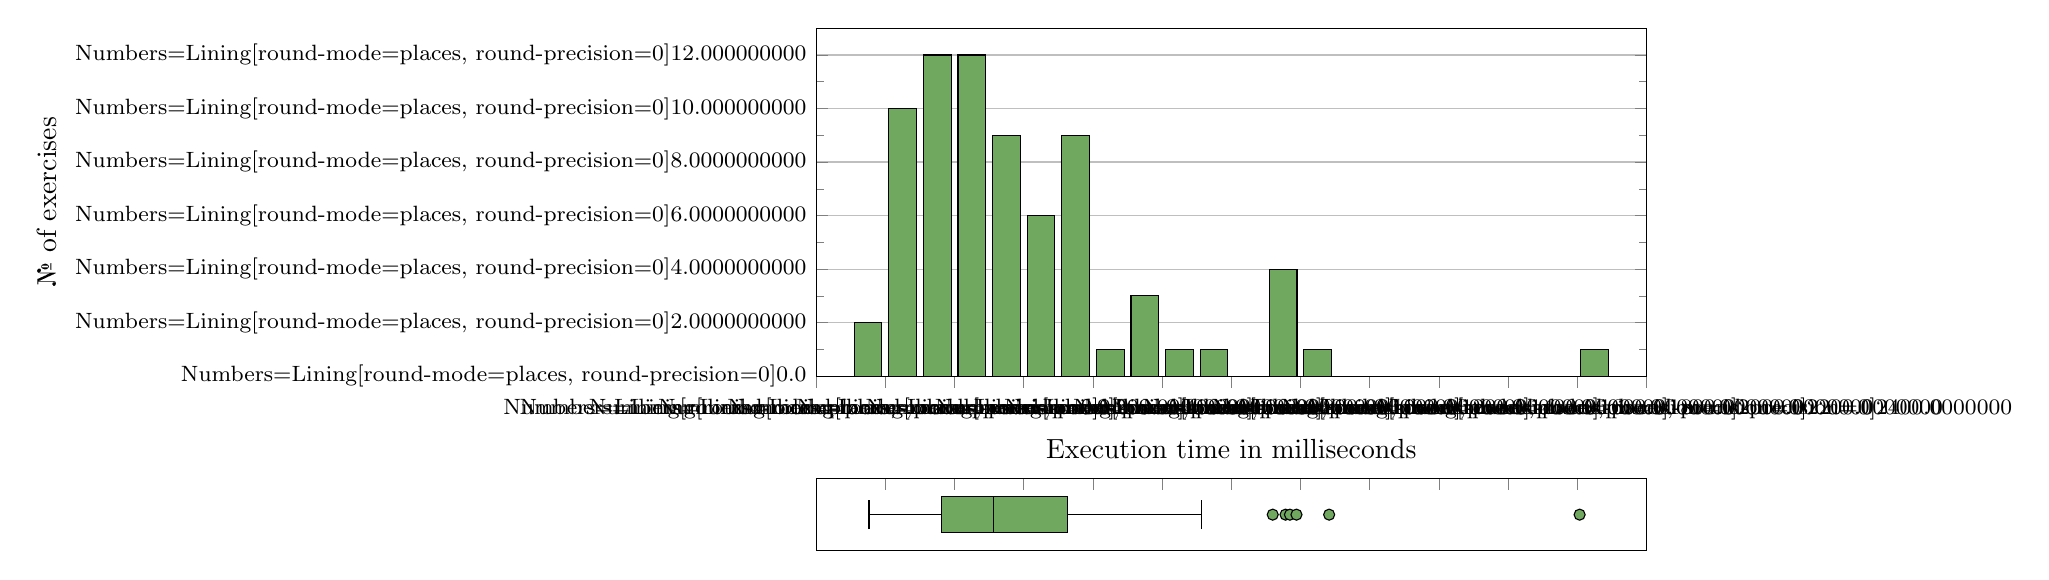
\begin{tikzpicture}
    \begin{axis}[
        ybar,
        ymin=0,
        ymax=13,
        ytick={0,2,...,13},
        minor y tick num=1,
        ymajorgrids,
        xmin=0,
        xtick={0,200,...,2400},
        xmax=2400,
        width=\textwidth,
        height=6cm,
        tick label style={font=\footnotesize},
        xlabel={Execution time in milliseconds},
        ylabel={\textnumero{} of exercises},
        xtick pos=left,
        name=hist,
        xticklabel={\addfontfeature{Numbers={Lining}}\num[round-mode=places, round-precision=0]{\tick}},
        yticklabel={\addfontfeature{Numbers={Lining}}\num[round-mode=places, round-precision=0]{\tick}}
    ]
        \addplot[fill=ugent-ps] coordinates {
            (150,2)
            (250,10)
            (350,12)
            (450,12)
            (550,9)
            (650,6)
            (750,9)
            (850,1)
            (950,3)
            (1050,1)
            (1150,1)
            (1350,4)
            (1450,1)
            (2250,1)
        };
    \end{axis}
    \begin{axis}[
        at={($(hist.south)-(0,1.3cm)$)},
        anchor=north,
        xmin=0,
        xtick={0,200,...,2400},
        xmax=2400,
        width=\textwidth,
        height=2.5cm,
        ytick=\empty,
        xtick pos=right,
        xticklabels=\empty,
        ymin=0.5, ymax=1.5
    ]
        \addplot [boxplot prepared={
            lower whisker=152.5999725,
            lower quartile=363.02634409999996,
            median=512.23714275,
            upper quartile=725.250321875,
            upper whisker=1113.508318,
            box extend=0.5
        },draw=black,fill=ugent-ps] coordinates {(0,1319.759644) (0,1356.797906) (0,1369.516804) (0,1388.407927) (0,1482.881139) (0,2206.955292)};
    \end{axis}
\end{tikzpicture}

\end{document}
